\section{Materials and Methods}\label{sec:method}

\subsection{Problem Setup}\label{subsec:problem_setup}

WaveletMask is built on the bidirectional recurrent propagation framework of RTN~\cite{rtn2022}. Given a degraded clip $\{I_t^{\mathrm{LQ}}\}_{t=1}^{T}$ with spatial resolution $H\times W$, the goal is to reconstruct restored frames $\{I_t^{\mathrm{HQ}}\}_{t=1}^{T}$ while suppressing both local structural damage and temporal photometric artifacts. Unless otherwise stated, the batch dimension $B$ is omitted in the equations. Input frames are represented as $I_t^{\mathrm{LQ}}\in\mathbb{R}^{3\times H\times W}$, luminance frames as $I_t^{\mathrm{gray}}\in\mathbb{R}^{1\times H\times W}$, and masks as single-channel tensors in $[0,1]^{1\times H\times W}$.

In the RTN, optical flow is estimated between adjacent frames with RAFT~\cite{teed2020raft}, and a warped pixel-domain difference is used as the degradation indicator. For propagation direction $d\in\{-1,+1\}$, the directed spatial indicator is
\begin{equation}\label{eq:baseline_indicator}
    r_{t,d}^{\mathrm{spatial}} = \left|\mathcal{W}\!\left(I_{t+d}^{\mathrm{LQ}},\phi_{t+d\to t}\right)-I_t^{\mathrm{LQ}}\right|_{Y},
\end{equation}
where $\mathcal{W}(\cdot,\cdot)$ denotes flow-based warping, $\phi_{t+d\to t}$ is the estimated optical flow, and $|\cdot|_{Y}$ denotes conversion to the luminance channel after the absolute RGB difference. High indicator values encourage the gated aggregation module to rely more on current-frame evidence, whereas low values encourage reuse of propagated features.

WaveletMask replaces this motion-sensitive spatial indicator with a frame-centered wavelet-domain mask computed from bilateral temporal evidence. The detector first predicts $m_t^{\mathrm{wavelet}}$ from the current frame and its temporal neighbors, and the same mask is then injected into both propagation directions:
\begin{equation}\label{eq:gate_mask}
    m_{t,d}^{\mathrm{gate}} = m_t^{\mathrm{wavelet}}, \quad d\in\{-1,+1\}.
\end{equation}
Using a shared gate mask for $d\in\{-1,+1\}$ matches the implementation and reflects the fact that the wavelet detector is anchored at frame $t$ rather than at a specific propagation direction. In the proposed model, $m_t^{\mathrm{wavelet}}$ is obtained from LHFM and GFM followed by element-wise maximum fusion. Learned variants that additionally combine the RTN spatial indicator with the wavelet mask are evaluated only as ablations in Appendix~\ref{subsec:fusion_analysis} and are not part of the final architecture.

\subsection{Pipeline Overview}\label{subsec:overview}

Figure~\ref{fig:pipeline} summarizes the final WaveletMask pipeline. For each frame, the WaveletNoiseMask block pre-computes a wavelet-domain gate mask from the current frame and its two temporal neighbors, and the resulting $m_t^{\mathrm{wavelet}}$ is injected directly into the forward and backward recurrent gates in Equation~\eqref{eq:gate_mask}. The restoration backbone, bidirectional propagation schedule, and training losses remain identical to RTN; only the gate input is changed.

\begin{figure}[t]
\centering
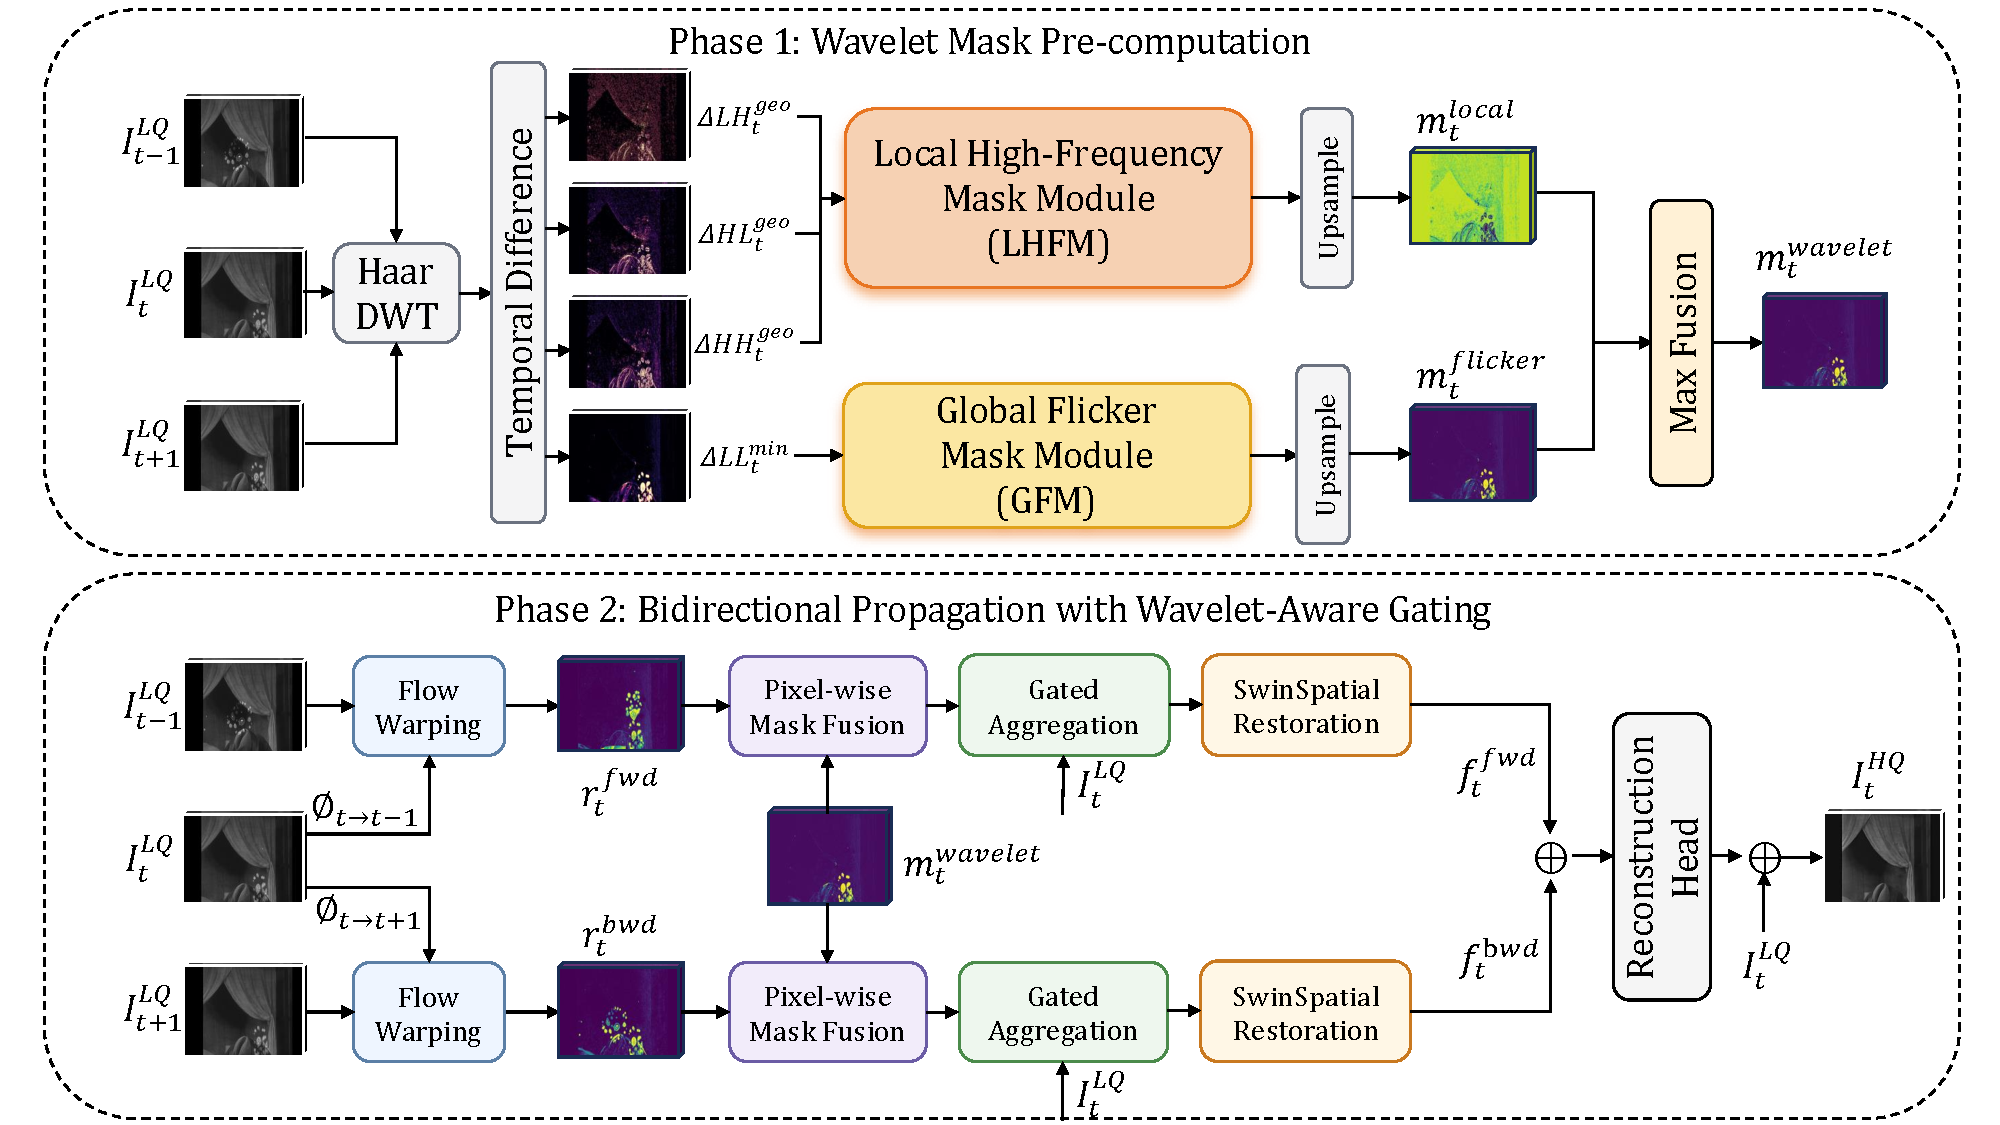
\includegraphics[width=\textwidth]{figures/Figure2.pdf}
\caption{Overview of the final WaveletMask pipeline. The WaveletNoiseMask module pre-computes the branch-max wavelet mask $m_t^{\mathrm{wavelet}}$ from neighboring frames, and the resulting mask is injected directly into the forward and backward recurrent gates. Learned CNN fusion variants that additionally use the RTN spatial indicator are ablated in Table~\ref{tab:fusion_comparison} and are not part of the proposed model.\label{fig:pipeline}}
\end{figure}

Unlike the flow-guided propagation path in RTN, the wavelet detector intentionally operates on raw temporal neighbors instead of motion-compensated ones. An auxiliary code path includes an optional flow-compensated wavelet variant, but this switch is disabled in the proposed model because a small pixel-domain misregistration perturbs multiple LL/LH/HL/HH coefficients after the discrete wavelet transform, thereby amplifying optical-flow errors into structured false responses near motion boundaries. For the same reason, the proposed model fixes a single-level Haar decomposition; alternative wavelet families and learned fusion variants are reserved for ablation-only experiments.

The recurrent aggregation step can be written as
\begin{equation}\label{eq:gated_agg}
    f_t^{\mathrm{agg}} = \mathrm{GatedAgg}\!\left(f_{\mathrm{prop}},I_t^{\mathrm{LQ}},m_{t,d}^{\mathrm{gate}}\right),
\end{equation}
where $m_{t,d}^{\mathrm{gate}}$ is broadcast along the feature-channel dimension. The reconstruction head follows the original RTN contract:
\begin{equation}\label{eq:reconstruction}
    I_t^{\mathrm{HQ}} = \tanh\!\left(\mathrm{Upsample}\!\left([f_t^{\mathrm{bwd}},f_t^{\mathrm{fwd}}]\right)+I_t^{\mathrm{LQ}}\right).
\end{equation}
Because the wavelet mask is pre-computed before recurrent propagation and the final fusion is parameter-free, the proposed variant changes only the gate input while leaving the restoration backbone, losses, and propagation structure unchanged.

\subsection{Local High-Frequency Mask Module (LHFM)}\label{subsec:local}

Unlike pixel-domain differences that entangle thin defects with motion boundaries and warping residuals, LHFM isolates transient local corruption by measuring bilateral consistency in the wavelet detail sub-bands. Figure~\ref{fig:lhfm} shows the module architecture.

\begin{figure}[t]
\centering
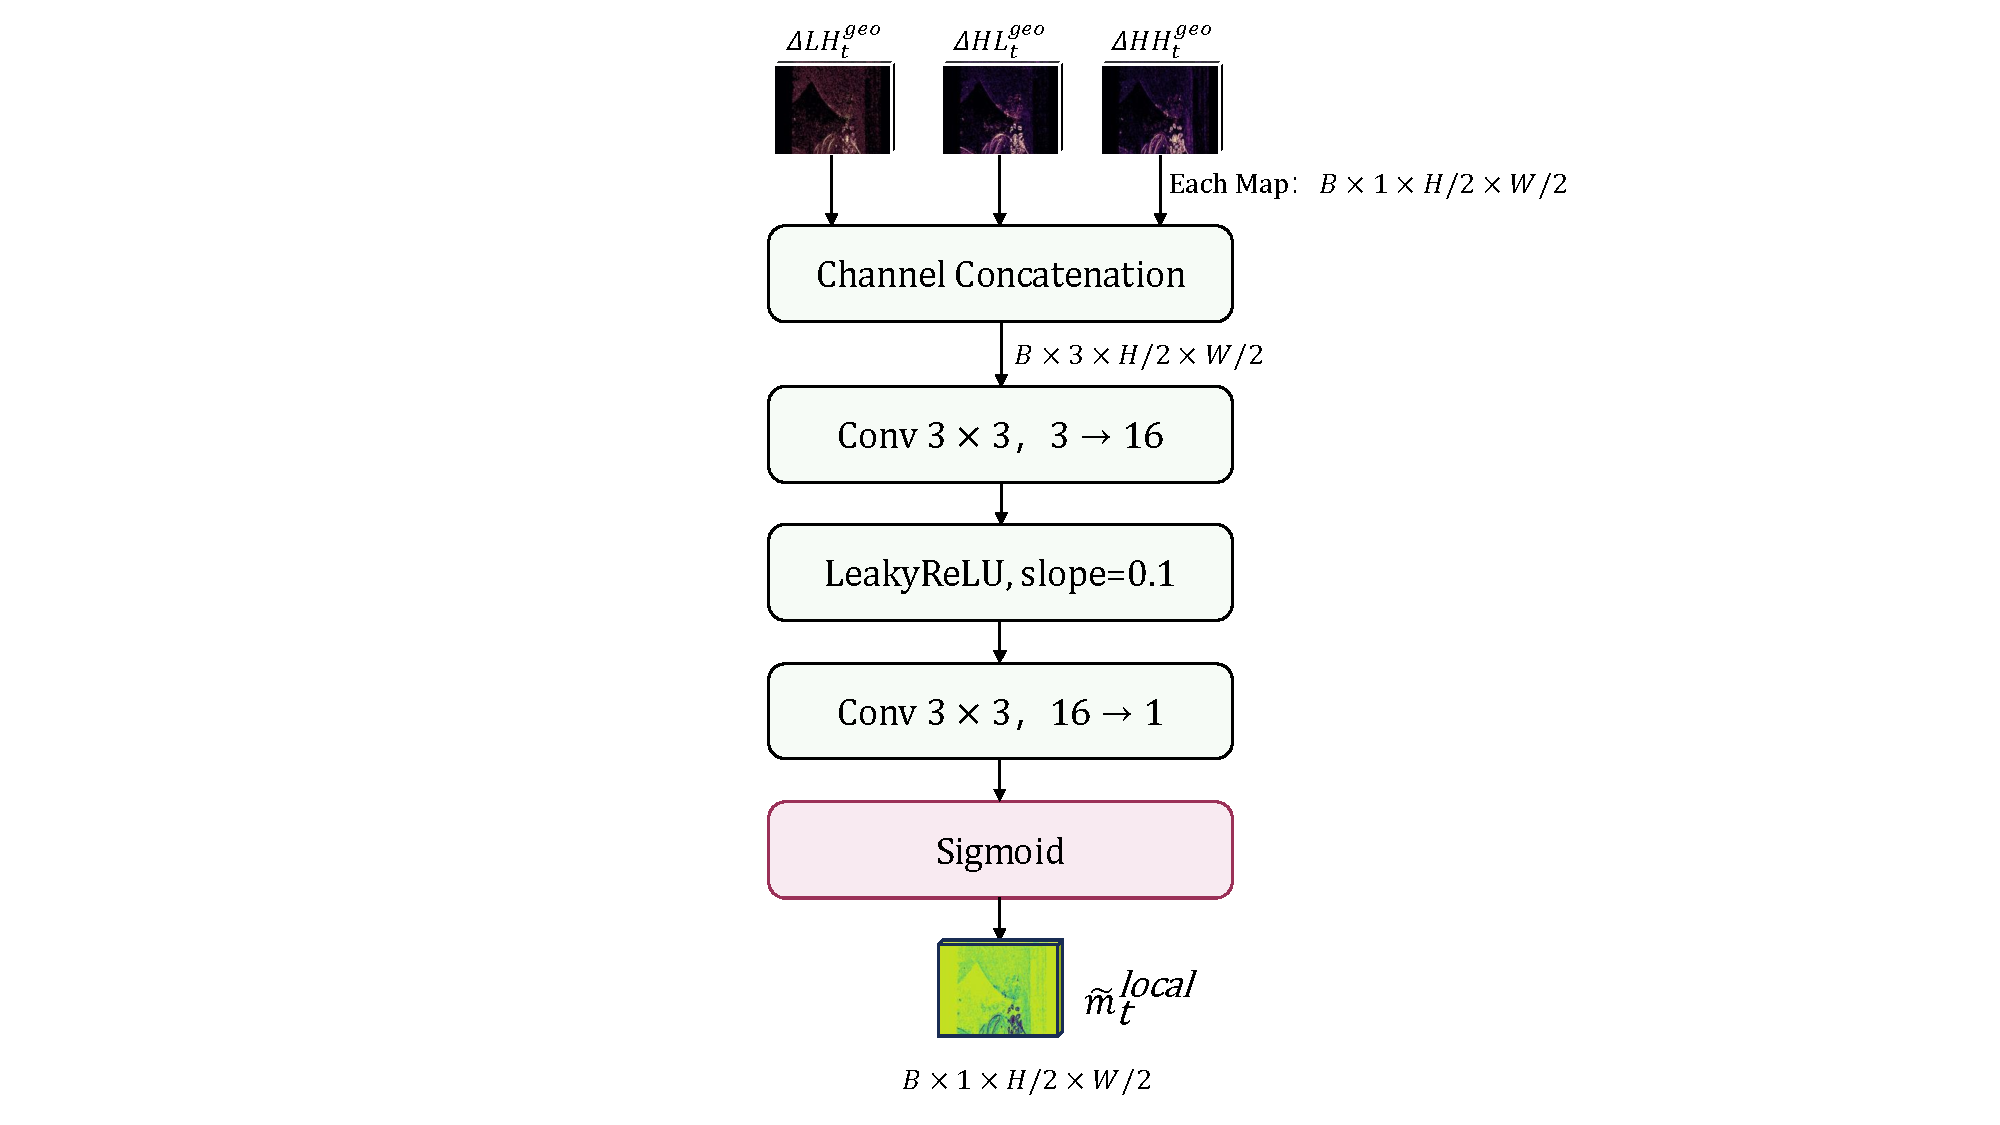
\includegraphics[width=\textwidth]{figures/Figure3.pdf}
\caption{LHFM architecture. Geometric-mean temporal differences from the LH, HL, and HH detail sub-bands are concatenated and processed by \texttt{high\_freq\_conv}, consisting of a 3$\times$3 3$\to$16 convolution, LeakyReLU, a 3$\times$3 16$\to$1 convolution, and sigmoid activation. The half-resolution output $\tilde{m}_t^{\mathrm{local}}\in[0,1]^{1\times H/2\times W/2}$ is bilinearly upsampled before fusion.\label{fig:lhfm}}
\end{figure}

Each RGB frame is first converted to luminance using the BT.601 transform, $I_t^{\mathrm{gray}}=0.299R+0.587G+0.114B$, and is then decomposed by a single-level Haar DWT:
\begin{equation}\label{eq:haar_dwt}
    \{\mathrm{LL}_t,\mathrm{LH}_t,\mathrm{HL}_t,\mathrm{HH}_t\}=\mathrm{HaarDWT2d}(I_t^{\mathrm{gray}}).
\end{equation}
Here, $\mathrm{LL}_t$ denotes the low-frequency approximation, while $\mathrm{LH}_t$, $\mathrm{HL}_t$, and $\mathrm{HH}_t$ denote the horizontal, vertical, and diagonal detail coefficients, respectively. The proposed model uses fixed $2\times2$ Haar analysis filters normalized by $1/2$, so the transform introduces no learnable parameters.

To suppress one-sided temporal residuals, LHFM requires simultaneous disagreement with both temporal neighbors. For each high-frequency sub-band $S\in\{\mathrm{LH},\mathrm{HL},\mathrm{HH}\}$, the bilateral response is computed as
\begin{equation}\label{eq:geomean}
    d_t^{S}=\sqrt{|S_t-S_{t^-}|\,|S_t-S_{t^+}|+\epsilon},
\end{equation}
where $t^-$ and $t^+$ denote the previous and next neighbors for non-boundary frames, and $\epsilon=10^{-8}$ is used for numerical stability. The geometric mean behaves like a bilateral ``and'' operator: if either temporal difference is small, the overall response remains small. Consequently, one-sided motion or warping residuals are attenuated, whereas a transient scratch or dust particle that differs from both neighbors produces a strong activation. Boundary frames do not have bilateral temporal evidence and are assigned zero wavelet masks. This design is effective for single-frame defects, but when a scratch persists across three or more consecutive frames at nearly the same image-plane position ($S_{t-1}\approx S_t\approx S_{t+1}$), both temporal differences vanish and $d_t^S\to 0$, suppressing the LHFM response (see Section~\ref{subsec:response_analysis} and Table~\ref{tab:persistent_scratch_probe}).

The three directional responses are then aggregated by a lightweight prediction head:
\begin{equation}\label{eq:local_mask}
    \tilde{m}_t^{\mathrm{local}}=\sigma\!\left(\mathrm{Conv}_{16\to1}\!\left(\mathrm{LeakyReLU}\!\left(\mathrm{Conv}_{3\to16}\!\left([d_t^{\mathrm{LH}},d_t^{\mathrm{HL}},d_t^{\mathrm{HH}}]\right)\right)\right)\right),
\end{equation}
where $\sigma$ denotes the sigmoid activation and $[\cdot]$ denotes channel-wise concatenation. The resulting half-resolution prediction is bilinearly upsampled to the image resolution:
\begin{equation}\label{eq:local_mask_up}
    m_t^{\mathrm{local}}=\mathrm{Up}(\tilde{m}_t^{\mathrm{local}}), \quad m_t^{\mathrm{local}}\in[0,1]^{1\times H\times W},
\end{equation}
where $\mathrm{Up}(\cdot)$ denotes bilinear upsampling.

\subsection{Global Flicker Mask Module (GFM)}\label{subsec:flicker}

Unlike pixel-domain differences that are dominated by edges, texture, and local motion, GFM captures frame-level photometric instability by measuring bilateral low-frequency deviations on the LL sub-band. Figure~\ref{fig:gfm} shows the module architecture.

After obtaining the LL coefficients, we compute the forward and backward low-frequency deviations as
\begin{equation}\label{eq:flicker_diff}
    d_t^{\mathrm{fwd}}=|\mathrm{LL}_t-\mathrm{LL}_{t^-}|,\quad d_t^{\mathrm{bwd}}=|\mathrm{LL}_t-\mathrm{LL}_{t^+}|.
\end{equation}
GFM then enforces bilateral agreement through a minimum operator:
\begin{equation}\label{eq:flicker_min}
    d_t^{\mathrm{flicker}}=\min(d_t^{\mathrm{fwd}},d_t^{\mathrm{bwd}}).
\end{equation}
The minimum rule is used instead of an average because a genuine flicker event should increase both forward and backward LL differences. If only one direction is large, the response is limited to the smaller value, which reduces sensitivity to one-sided brightness changes. At the same time, abrupt scene cuts, flashes, and other broad illumination changes can also elevate both LL differences. These failure modes are quantified in Table~\ref{tab:gfm_failure_probe} and discussed in Section~\ref{subsec:response_analysis}.

\begin{figure}[H]
\centering
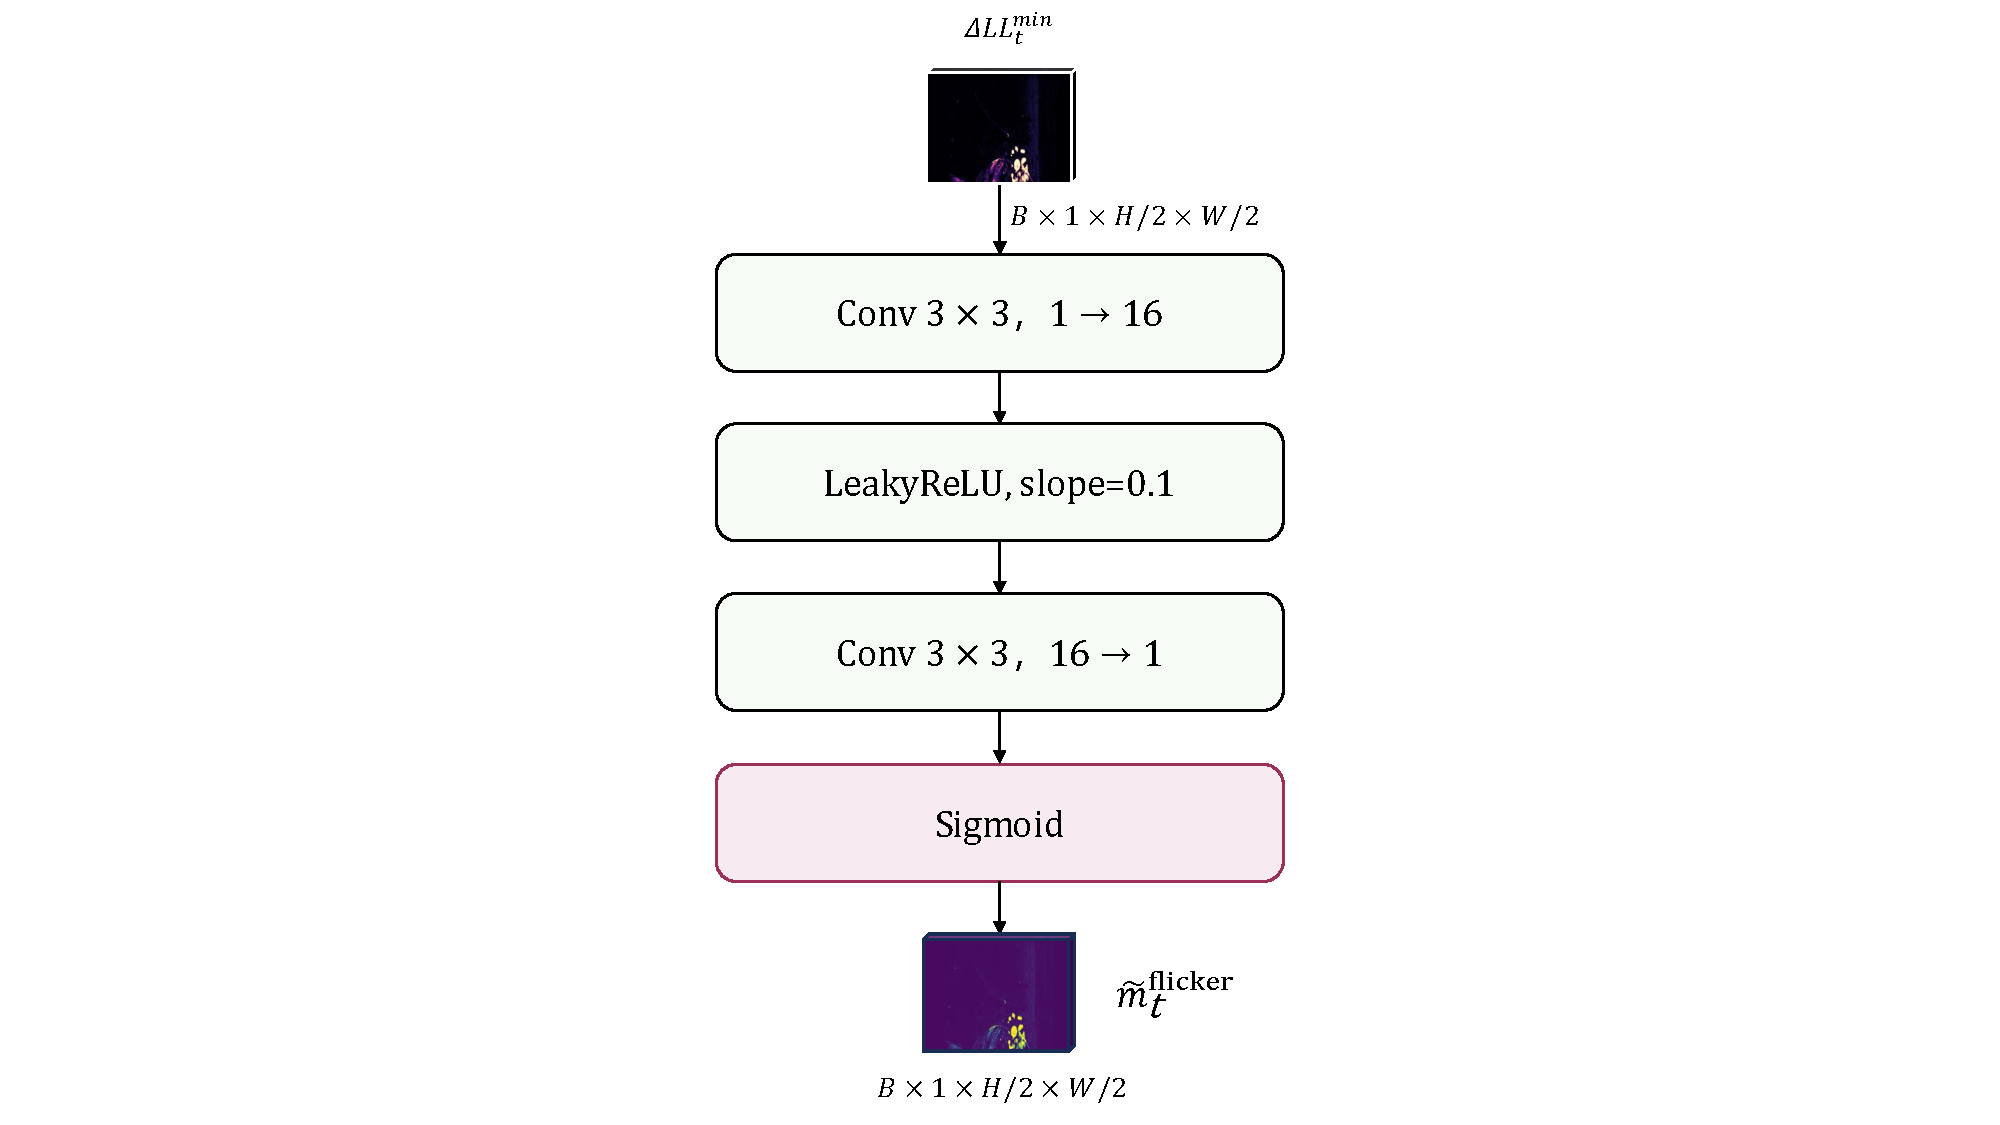
\includegraphics[width=\textwidth]{figures/Figure4.pdf}
\caption{GFM architecture. The minimum LL temporal response is processed by \texttt{low\_freq\_conv}, consisting of a 3$\times$3 1$\to$16 convolution, LeakyReLU, a 3$\times$3 16$\to$1 convolution, and sigmoid activation. The half-resolution output $\tilde{m}_t^{\mathrm{flicker}}\in[0,1]^{1\times H/2\times W/2}$ is bilinearly upsampled before fusion.\label{fig:gfm}}
\end{figure}

The low-frequency response is decoded by a second lightweight prediction head:
\begin{equation}\label{eq:flicker_mask}
    \tilde{m}_t^{\mathrm{flicker}}=\sigma\!\left(\mathrm{Conv}_{16\to1}\!\left(\mathrm{LeakyReLU}\!\left(\mathrm{Conv}_{1\to16}(d_t^{\mathrm{flicker}})\right)\right)\right),
\end{equation}
followed by bilinear upsampling to the original resolution:
\begin{equation}\label{eq:flicker_mask_up}
    m_t^{\mathrm{flicker}}=\mathrm{Up}(\tilde{m}_t^{\mathrm{flicker}}), \quad m_t^{\mathrm{flicker}}\in[0,1]^{1\times H\times W}.
\end{equation}

\subsection{Mask Fusion and Integration}\label{subsec:integration}

Unlike pixel-domain differences that collapse local scratches and global luminance shifts into a single motion-sensitive residual, the integration stage preserves whichever wavelet branch provides the stronger evidence at each pixel. As further clarified in Section~\ref{subsec:response_analysis}, LHFM and GFM are complementary rather than redundant, so the fusion rule should avoid attenuating a decisive single-branch response.

WaveletMask therefore uses a branch-level maximum operation:
\begin{equation}\label{eq:wavelet_mask}
    m_t^{\mathrm{wavelet}}=\max(m_t^{\mathrm{local}},m_t^{\mathrm{flicker}}).
\end{equation}
The element-wise maximum treats local structural damage and global flicker as alternative degradation evidence: if either branch fires, the wavelet mask is activated. This choice also matches the implementation exactly, where $\max(\cdot,\cdot)$ is used directly after the two mask heads. Compared with learned convex fusion, this rule preserves a strong activation from either branch instead of averaging it with a weak companion response. The ablation results in Table~\ref{tab:fusion_comparison} further show that parameter-free max fusion is preferable to learned PixelWiseMaskFusion, which supports the final design choice.

The complete detector consists of the fixed Haar DWT and two lightweight CNN heads, introducing only 898 learnable detector parameters. By contrast, the learned PixelWiseMaskFusion ablation adds 14,497 additional fusion parameters and also mixes in the RTN spatial indicator. These learned spatial--wavelet fusion variants are therefore treated as ablations rather than components of the final WaveletMask model.

\subsection{Response Analysis}\label{subsec:response_analysis}

To clarify the design rationale and boundary conditions of LHFM and GFM, we analyze several canonical temporal patterns.

\textbf{Local high-frequency response.} Equation~\eqref{eq:geomean} is designed to respond strongly only when the current high-frequency coefficient differs from both temporal neighbors. For a single-frame transient scratch at time $t$ ($S_{t-1}=0,\;S_t>0,\;S_{t+1}=0$), both terms under the geometric mean are large, producing the intended strong $d_t^S$ response. If only one directional difference is elevated, the product remains limited, which explains why the geometric mean suppresses one-sided motion or warping residuals more effectively than a simple sum or average. Conversely, for a persistent fixed scratch spanning $\geq$3 frames ($S_{t-1}\approx S_t\approx S_{t+1}$), both temporal differences vanish and $d_t^S\to0$, suppressing the LHFM response. This is an inherent boundary condition of the bilateral design: persistent image-plane-fixed scratches are progressively attenuated with increasing persistence length (46\% suppression at $L=2$, 65\% at $L\geq3$; see Table~\ref{tab:persistent_scratch_probe}). Drifting scratches that shift spatially between frames break the equality condition and are therefore not suppressed in the same way.

\textbf{Global flicker response.} Equation~\eqref{eq:flicker_min} similarly enforces bilateral agreement, but on the low-frequency LL component. A valid flicker event causes both forward and backward LL differences to increase, so the minimum remains high; this is why the minimum rule is better aligned with frame-level flicker than an average that can be dominated by a single-sided deviation. However, scene cuts and exposure flashes also produce bilateral LL elevation. In our probes, a scene cut yields $2.35\times$ baseline activation, and a flash yields $10.41\times$ (Table~\ref{tab:gfm_failure_probe}). A luminance-difference guard can suppress 61\% of scene-cut and 95\% of flash false responses, but it is not integrated into the current model in order to keep the proposed detector lightweight and scope-consistent.

Taken together, these complementary response patterns explain the integration strategy in Section~\ref{subsec:integration}: the final gate should preserve the stronger local or global cue at each pixel, rather than learn an averaging rule that may dilute a decisive single-branch response.

\subsection{Training Objective}\label{subsec:training}

Training follows the RTN protocol~\cite{rtn2022}. The total objective is
\begin{equation}\label{eq:loss_total}
    \mathcal{L}_{\mathrm{total}}=\mathcal{L}_{\mathrm{pix}}+\lambda_{\mathrm{perc}}\mathcal{L}_{\mathrm{perc}}+\lambda_{\mathrm{gan}}\mathcal{L}_{\mathrm{gan}},
\end{equation}
where $\mathcal{L}_{\mathrm{pix}}$ is an $L_1$ reconstruction loss, $\mathcal{L}_{\mathrm{perc}}$ is a VGG-based perceptual loss~\cite{johnson2016perceptual,simonyan2014vgg}, and $\mathcal{L}_{\mathrm{gan}}$ is a non-saturating adversarial loss~\cite{goodfellow2014gan}. The weights are $\lambda_{\mathrm{perc}}=1.0$ and $\lambda_{\mathrm{gan}}=0.01$, following RTN~\cite{rtn2022}. No explicit mask supervision is used; the wavelet branches and the restoration backbone are optimized only through the restoration losses. This choice preserves compatibility with the baseline training loop, but it also limits how strongly the learned masks can be interpreted as ground-truth artifact segmentations.
